\documentclass[12pt,a4paper]{article}

% Margins.
\setlength{\oddsidemargin}{0in}
\setlength{\evensidemargin}{0in}
\setlength{\headheight}{12pt}
\setlength{\headsep}{42pt}
\setlength{\topmargin}{-54pt}
\setlength{\textwidth}{6.5in}
\setlength{\textheight}{10in}

\usepackage{amsmath}
\usepackage{float}
\usepackage{graphicx}
\usepackage[hyphens]{url}
\usepackage{hyperref}	% Clickable links to figures, references and urls.
\usepackage{datetime}
\usepackage{longtable}
\usepackage{subfigure}

% Links direct to top of figures.
\usepackage[all]{hypcap}

% Drawing.
\usepackage{pgf}
\usepackage{tikz}

% Listings for formatting code.
\usepackage{listings}
\usepackage{textcomp}
% General options.+++
\lstset{breaklines=true, basicstyle=\small\ttfamily, tabsize=4, numbers=left, stepnumber=1, frame=single, showstringspaces=false, upquote=true}
% C++ specific high-lighting. Comments are 50/50 shades of green/black and strings coloured with 60/40 red/black mixture.
\lstset{language=[ISO]C++, commentstyle=\color{green!50!black}, keywordstyle=\color{blue}, stringstyle=\color{red!60!black}}

%opening
\title{\vspace{-2cm}Physics for Engineers\\Class 14\\Coulomb's Law: Problems}
\author{Attique Dawood}
\date{September 18, 2013\\[0.2cm] Last Modified: \today, \currenttime}
\begin{document}
\maketitle
\section{Announcements}
\begin{itemize}
\item Assignment 03 is due today.
\end{itemize}
\section{Revision}
\begin{itemize}
\item Vector and magnitude form of Coulomb's Law.
\end{itemize}
\section{Coulomb's Law}
Force exerted by a charge $q_1$ on another charge $q_2$ can be calculated using Coulomb's Law.
\begin{equation}
\textbf{F}_{12}=\dfrac{q_1q_2}{4\pi\epsilon_0 |\textbf{r}_2-\textbf{r}_1|^3}(\textbf{r}_2-\textbf{r}_1)
\end{equation}
Here $\textbf{r}_1$ and $\textbf{r}_2$ are position vectors of charges $q_1$ and $q_2$, respectively.
The magnitude of Coulombic force is given by the seldom used formula
\begin{equation}
\mathrm{F}_{12}=\dfrac{|q_1||q_2|}{4\pi\epsilon_0r^2}
\end{equation}
\newpage
\section{Exercises}
\noindent\textbf{Question 1 \cite[Example 23.2, page 713]{Serway}:} Three charges are located at the corners of a right angle triangle as shown in figure \ref{Resultant-force}. Here $q_1=q_3=5~\mu$C, $q_2=-2~\mu$C and $a=0.1$ m. Find the force on $q_1$, $q_2$ and $q_3$.
\begin{figure}[H]
\centering
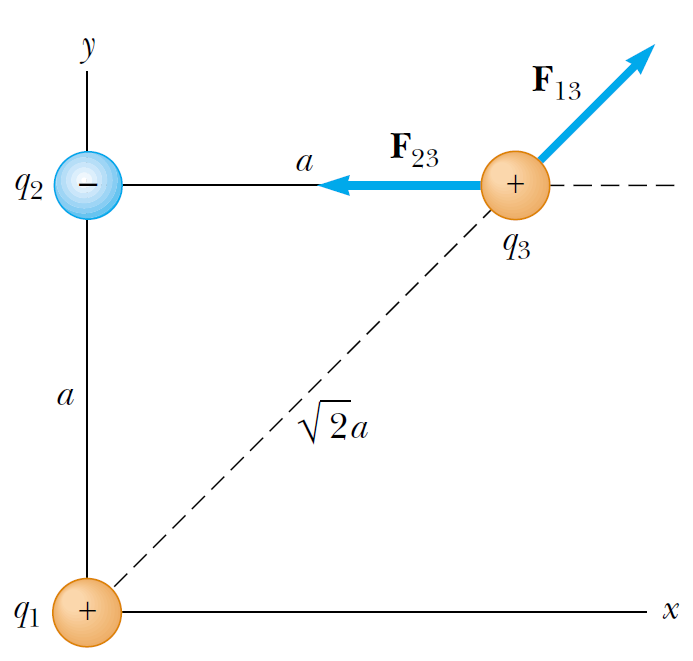
\includegraphics[scale=0.5]{Figure23-8.png}
\caption{Finding resultant force on a charge.}
\label{Resultant-force}
\end{figure}
\noindent\textbf{Question 2 \cite[Example 23.3, page 714]{Serway}:} Three charges are located in a straight line as shown in figure \ref{Zero-force}. Here $q_1=15~\mu$C and $q_2=6~\mu$C. Given that resultant force on $q_3$ is zero find the location of $q_3$.
\begin{figure}[H]
\centering
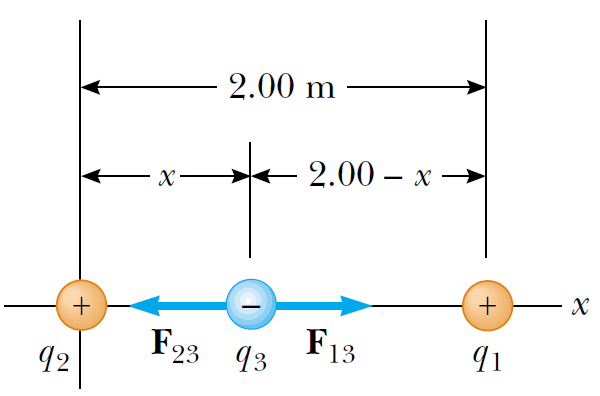
\includegraphics[scale=0.6]{Figure23-9.png}
\caption{Where is resultant force zero?}
\label{Zero-force}
\end{figure}
%\nocite{*}
\bibliographystyle{plain}
\bibliography{PhysicsRef}
\end{document}
